% Sección 4, Juan Diego · Se incluye desde informe.tex. Parte de primera_entrega.tex (etiqueta entrega-1).

\section{Recolección y entendimiento de datos}\label{sec:datos}

\subsection{Fuentes y procedimiento de recolección}

Se usan tres fuentes oficiales, cada una con una función distinta en el proyecto (tabla~\ref{tab:fuentes}): los archivos anuales de delitos a nivel de registro de la Policía Nacional \citep{policia}, el conjunto \emph{Procesos Fiscalía V3} \citep{fiscalia} y las llamadas tramitadas por la Línea 123 \citep{linea123}. Los archivos se descargaron sin modificar entre el 9 y el 12 de noviembre de 2026 y se conservan fuera del repositorio. Para cada uno se registran la URL, la fecha de extracción y el SHA-256 (apéndice~\ref{ap:archivos}).

Todas las cifras de esta sección provienen de scripts versionados en el repositorio del proyecto:
\begin{itemize}
  \item \texttt{scripts/auditoria\_datasets.py} calcula el embudo de filtros, los nulos, los duplicados y la cobertura (\texttt{outputs/auditoria/} y \texttt{outputs/auditoria\_policia/});
  \item \texttt{scripts/serie\_objetivo\_policia.py} construye la serie objetivo; sus salidas están en \texttt{outputs/serie\_objetivo/};
  \item \texttt{scripts/fiscalia\_modalidades.py} y \texttt{scripts/figuras\_informe.py} producen las tablas y figuras complementarias (\texttt{outputs/informe/}).
\end{itemize}
El procedimiento para reproducirlas está en \texttt{docs/AUDITORIA.md}.

{\small
\setlength{\tabcolsep}{4pt}
\begin{longtable}{@{}>{\raggedright\arraybackslash}p{2.5cm}>{\raggedright\arraybackslash}p{3.3cm}>{\raggedright\arraybackslash}p{3.8cm}>{\raggedright\arraybackslash}p{2.0cm}>{\raggedright\arraybackslash}p{3.2cm}@{}}
\caption{Fuentes del proyecto y función de cada una.}\label{tab:fuentes}\\
\toprule
\textbf{Fuente} & \textbf{Función} & \textbf{Unidad de la fila} & \textbf{Periodo} & \textbf{Filas de hurto en Bogotá} \\
\midrule
\endfirsthead
\toprule
\textbf{Fuente} & \textbf{Función} & \textbf{Unidad de la fila} & \textbf{Periodo} & \textbf{Filas de hurto en Bogotá} \\
\midrule
\endhead
\bottomrule
\endfoot
Policía Nacional, registro & Principal: requisito de volumen y variable objetivo & Una víctima de hurto a personas (\texttt{CANTIDAD} = 1) & 2020--2025 & 741.986 \\
\addlinespace
Fiscalía, Procesos V3 & Complementaria: respuesta judicial & Un par proceso--delito, capítulo «Del Hurto», todas las modalidades & 2018--2025 & 1.300.703 (991.471 en 2020--2025) \\
\addlinespace
Línea 123 & Complementaria: demanda ciudadana y territorio & Conteo de llamadas por año, mes, localidad, UPZ y tipo de incidente & 2018--2025 & 25.144 filas que suman 1.094.313 llamadas (19.286 y 821.304 en 2020--2025) \\
\addlinespace
MinDefensa, agregado diario & Contexto 2018--2019 y control de consistencia & Conteo de hurtos por día y municipio & 2018--2025 & 2.922 días que suman 975.793 hurtos \\
\end{longtable}
}

\subsection{Requisito mínimo de 500.000 registros}

El requisito se cumple con una sola fuente y una sola unidad de observación: el registro de hurto a personas de la Policía Nacional, en el que cada fila es una víctima. La tabla~\ref{tab:embudo} muestra el embudo de filtros sobre los seis archivos anuales. Las filas de fuentes distintas no se suman, porque una misma situación puede generar a la vez una llamada, un registro policial y un proceso judicial.

\begin{table}[H]
\centering
\caption{Embudo de filtros del registro de la Policía Nacional, 2020--2025.}\label{tab:embudo}
\begin{tabular}{@{}lr@{}}
\toprule
\textbf{Etapa} & \textbf{Filas} \\
\midrule
Seis archivos anuales, todo el país y todos los delitos & 4.829.870 \\
Bogotá (\texttt{CODIGO DANE} = 11001) & 1.406.157 \\
Hurto a personas (\texttt{DELITOS} = «(05022) Hurto a personas») & \textbf{741.986} \\
\bottomrule
\end{tabular}
\end{table}

La cifra está verificada de tres maneras:
\begin{enumerate}
  \item \textbf{Dos descargas independientes.} Los seis archivos, descargados por separado el 11 y el 12 de noviembre de 2026, tienen el mismo SHA-256. Las dos ejecuciones de la auditoría producen el mismo embudo, los mismos nulos y los mismos duplicados.
  \item \textbf{La unidad es individual.} \texttt{CANTIDAD} vale 1 en todas las filas, así que el número de filas coincide con la suma de víctimas.
  \item \textbf{Concordancia con el agregado de MinDefensa.} En 2020--2025 el agregado diario suma 741.987 hurtos: cinco de los seis años coinciden exactamente, y la diferencia de un registro se concentra en siete días de marzo de 2024 que se compensan entre sí.
\end{enumerate}

Conviene distinguir dos cantidades que se documentan por separado:
\begin{itemize}
  \item el \textbf{conjunto original}, de 741.986 filas, es el que sostiene el requisito;
  \item el \textbf{conjunto de modelamiento} es la serie diaria obtenida al agregar esas filas: 2.192 observaciones (sección~\ref{sec:objetivo}).
\end{itemize}
Que la serie tenga menos de 500.000 observaciones no cambia el volumen de la fuente.

\begin{table}[H]
\centering
\caption{Víctimas de hurto a personas registradas en Bogotá por año.}\label{tab:anual}
\begin{tabular}{@{}lrrrrrr@{}}
\toprule
 & \textbf{2020} & \textbf{2021} & \textbf{2022} & \textbf{2023} & \textbf{2024} & \textbf{2025} \\
\midrule
Registros (víctimas) & 83.136 & 109.428 & 137.157 & 158.745 & 130.503 & 123.017 \\
Media diaria & 227,15 & 299,80 & 375,77 & 434,92 & 356,57 & 337,03 \\
\bottomrule
\end{tabular}
\end{table}

\subsection{Fuente principal: Policía Nacional, delitos a nivel de registro}

La Policía publica un archivo anual con todos los delitos del país, una fila por víctima. Los años 2020 a 2025 están disponibles a este nivel; 2018 y 2019 no. El formato cambia entre años: el encabezado está en la fila 12 o en la 13, la columna del arma se llama \texttt{ARMA MEDIO} en 2021, y el archivo de 2023 no trae la columna \texttt{ICCS}. El conversor detecta el encabezado, descarta las 25.207 filas de notas del pie y unifica el nombre del arma. El filtro de hurto usa \texttt{DELITOS}, que existe en los seis años con la misma etiqueta. La tabla~\ref{tab:variables-policia} resume las variables tal como aparecen en los archivos y su perfil dentro de la población de 741.986 filas. El diccionario de las demás fuentes está en el apéndice~\ref{ap:diccionario}.

{\small
\setlength{\tabcolsep}{4pt}
\begin{longtable}{@{}>{\raggedright\arraybackslash}p{3.3cm}>{\raggedright\arraybackslash}p{1.8cm}>{\raggedright\arraybackslash}p{10.2cm}@{}}
\caption{Variables del registro de la Policía en la población de hurto a personas en Bogotá.}\label{tab:variables-policia}\\
\toprule
\textbf{Columna} & \textbf{Tipo} & \textbf{Contenido y perfil} \\
\midrule
\endfirsthead
\toprule
\textbf{Columna} & \textbf{Tipo} & \textbf{Contenido y perfil} \\
\midrule
\endhead
\bottomrule
\endfoot
\texttt{FECHA HECHO} & Fecha & Día del hecho (AAAA/MM/DD), sin hora. Sin nulos; los 2.192 días del periodo tienen al menos un registro. \\
\texttt{DEPARTAMENTO}, \texttt{MUNICIPIO}, \texttt{CODIGO DANE} & Texto & Ubicación hasta el municipio. No hay localidad, barrio ni coordenadas. \\
\texttt{DELITOS} & Categórico & Tipo de delito; el filtro conserva «(05022) Hurto a personas». \\
\texttt{ARMAS MEDIOS} & Categórico & Ocho categorías, sin nulos: sin empleo de armas (468.806; 63,2\,\%), arma blanca o cortopunzante (151.687; 20,4\,\%), arma de fuego (78.303; 10,6\,\%), contundentes (21.131), no reportado (15.558), escopolamina (6.449) y dos residuales. \\
\texttt{GENERO} & Categórico & Masculino (435.289; 58,7\,\%) y femenino (306.075; 41,3\,\%); 622 nulos (0,08\,\%). \\
\texttt{*AGRUPA EDAD PERSONA*} & Categórico & Tres grupos: 18 años y más (733.946; 98,9\,\%), 14 a 17 (6.609) y 0 a 14 (1.039); 392 nulos (0,05\,\%). \\
\texttt{MES} & Numérico & Mes del hecho, redundante con la fecha. \\
\texttt{CANTIDAD} & Numérico & Vale 1 en todas las filas. \\
\texttt{ICCS} & Texto & Código de la clasificación internacional del delito; ausente en 2023, no se usa. \\
\end{longtable}
}

Dos rasgos de esta fuente condicionan su tratamiento:
\begin{itemize}
  \item \textbf{Filas idénticas legítimas.} El archivo no publica identificador de víctima ni de hecho, así que dos víctimas del mismo día con el mismo arma, género y grupo de edad producen filas idénticas. Por eso 713.344 de las 741.986 filas repiten otra fila, y \textbf{no se eliminan}: quitarlas dejaría 28.642 filas y borraría víctimas reales. El control de consistencia de esta fuente es el agregado de MinDefensa, no la unicidad de filas.
  \item \textbf{Variables de la víctima sin validar.} El pie del archivo advierte que el género y la edad no tienen calidad validada en completitud. En Bogotá sus nulos son mínimos, pero la advertencia se mantiene como limitación.
\end{itemize}

\subsection{Fuente complementaria: Fiscalía, Procesos V3}

El conjunto \emph{Procesos Fiscalía V3} contiene las noticias criminales del Sistema Penal Oral Acusatorio. Se descargó con la API de datos.gov.co filtrando Bogotá (\texttt{cod\_dane\_hecho} = 11001) y el capítulo «Del Hurto». La auditoría da 2.002.177 filas en total y 1.300.703 con año del hecho entre 2018 y 2025. Esas filas corresponden a 1.297.042 procesos distintos, porque un proceso puede tener varios delitos: hay 3.661 filas repetidas, de 3.094 procesos.

La columna \texttt{delito} registra el tipo penal, es decir, el artículo del Código Penal, la cuantía y, si la hay, la circunstancia de agravación. No registra la víctima. Por eso \textbf{no es posible aislar el hurto a personas en esta fuente} (tabla~\ref{tab:fiscalia}):
\begin{itemize}
  \item el texto solo permite excluir 123.506 filas de modalidades identificables, como los vehículos o los establecimientos públicos;
  \item de las 1.177.197 restantes, 1.108.399 (94,2\,\%) son tipos genéricos, como «Hurto. Art. 239 C.P.», en los que van juntos el hurto a personas, a residencias y a comercio.
\end{itemize}

\begin{table}[H]
\centering
\small
\caption{Filas de Fiscalía 2018--2025 según la modalidad que nombra la columna \texttt{delito}.}\label{tab:fiscalia}
\begin{tabularx}{\textwidth}{@{}Xrr@{}}
\toprule
\textbf{Grupo} & \textbf{Filas} & \textbf{\%} \\
\midrule
Tipos genéricos sin modalidad (art. 239 y 240, con o sin cuantía) & 1.108.399 & 85,22 \\
Otros tipos no excluibles (agravantes que no nombran el objeto) & 68.798 & 5,29 \\
Medios motorizados o lo que transporten (art. 241, num. 6) & 59.616 & 4,58 \\
Establecimiento público (art. 241, num. 11) & 53.162 & 4,09 \\
Automotores & 10.558 & 0,81 \\
Abigeato, predio rural, objetos especiales y sin detalle & 170 & 0,01 \\
\midrule
Total & 1.300.703 & 100,00 \\
\bottomrule
\end{tabularx}
\end{table}

En consecuencia, las cifras de Fiscalía se citan siempre como «hurto en todas sus modalidades» y no se comparan en magnitud con el hurto a personas de la Policía. Esta fuente se usa para comparar tendencias, analizar la evolución de las noticias criminales y estudiar las diferencias entre el registro policial y el judicial. Sus filas no se interpretan como víctimas ni como hechos únicos. La fecha que se usa es la del hecho (año y mes). Del total descargado, 767 filas no la traen y quedan fuera del periodo; la fecha de creación del proceso no la sustituye.

\subsection{Fuente complementaria: Línea 123}

El recurso de llamadas tramitadas del C4 publica conteos agregados: cada fila suma las llamadas de un año, un mes, una localidad, una UPZ y un tipo de incidente en la columna \texttt{CANT\_INCIDENTES}. El archivo tiene 1.117.394 filas de 2015 a 2026, 763.074 de ellas en 2018--2025. Las de tipos de incidente con «HURTO» son 25.144 y suman 1.094.313 llamadas. En el periodo principal son 19.286 filas que suman 821.304 llamadas.

En esta fuente el volumen es la suma de \texttt{CANT\_INCIDENTES}, no el número de filas, y la columna \texttt{ID} no es única (166 identificadores repetidos entre las filas de hurto). Es la única fuente con resolución territorial dentro de la ciudad: 20 localidades y 116 UPZ, más valores sin ubicación («SIN LOCALIZACION», «SIN UPZ \ldots» y «-»). La figura~\ref{fig:localidad} muestra la distribución por localidad, y la tabla~\ref{tab:localidad-ap} da sus valores. Kennedy, Engativá y Suba concentran el 34,9\,\% de las llamadas de hurto de 2020--2025, y las llamadas sin localización son el 0,69\,\%. Esta distribución describe la demanda de atención y no se contrasta con las otras fuentes, que no identifican la localidad.

\begin{figure}[H]
\centering
\IfFileExists{figuras/linea123_localidad.pdf}{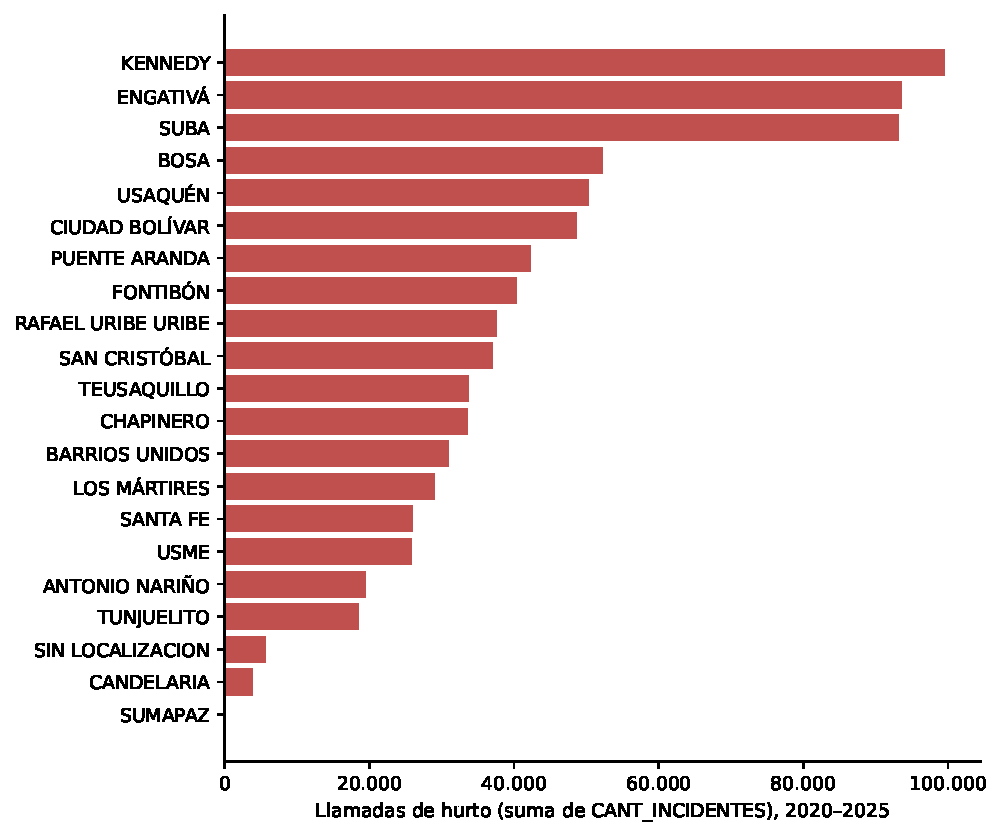
\includegraphics[width=0.78\textwidth]{figuras/linea123_localidad.pdf}}{\fbox{Figura pendiente: \texttt{figuras/linea123\_localidad.pdf}}}
\caption{Llamadas de hurto a la Línea 123 por localidad, 2020--2025 (suma de \texttt{CANT\_INCIDENTES}). Fuente: \texttt{outputs/informe/linea123\_localidad\_2020\_2025.csv}.}\label{fig:localidad}
\end{figure}

\subsection{Calidad de los datos}

La tabla~\ref{tab:calidad} resume los hallazgos de calidad de la población que usa cada fuente. Lo que la auditoría marca como anomalía no siempre es un error: varias marcas son rasgos de la fuente que se documentan, no se corrigen.

{\small
\setlength{\tabcolsep}{4pt}
\begin{longtable}{@{}>{\raggedright\arraybackslash}p{2.2cm}>{\raggedright\arraybackslash}p{6.6cm}>{\raggedright\arraybackslash}p{6.5cm}@{}}
\caption{Hallazgos de calidad y tratamiento previsto.}\label{tab:calidad}\\
\toprule
\textbf{Fuente} & \textbf{Hallazgo} & \textbf{Tratamiento} \\
\midrule
\endfirsthead
\toprule
\textbf{Fuente} & \textbf{Hallazgo} & \textbf{Tratamiento} \\
\midrule
\endhead
\bottomrule
\endfoot
Policía & 713.344 filas idénticas a otra, por falta de identificador & No deduplicar; controlar con el agregado diario \\
\addlinespace
Policía & Nulos: 622 en género (0,08\,\%) y 392 en grupo de edad (0,05\,\%); ninguno en fecha ni en arma & No imputar; tratar el nulo como categoría «no reportado» \\
\addlinespace
Policía & Caída abrupta en noviembre y diciembre de 2025: 5.416 y 5.700 víctimas, frente a 12.228 en octubre. Las mismas cifras aparecen en el agregado de MinDefensa y en los cuadros de salida validados de la Policía, y el hurto a residencias y a comercio de Bogotá cae en los mismos meses & Causa no establecida (issue \#86). Hasta aclararla, esos meses no se usan para evaluar modelos y no se interpretan como un descenso real \\
\addlinespace
Fiscalía & 3.661 filas repetidas, de 3.094 procesos con varios delitos & Contar filas o procesos según el análisis, declarándolo \\
\addlinespace
Fiscalía & 767 filas del total descargado sin fecha del hecho & Quedan fuera del periodo; no se imputan \\
\addlinespace
Fiscalía & Modalidad no identificable en el 94,2\,\% de las filas no excluibles & Citar como hurto en todas sus modalidades \\
\addlinespace
Línea 123 & \texttt{ID} repetido en 166 filas de hurto & No usar \texttt{ID} como clave \\
\addlinespace
Línea 123 & Valores sin ubicación en localidad y UPZ & Separarlos antes de cualquier análisis territorial \\
\end{longtable}
}

\subsection{Cobertura temporal}

La figura~\ref{fig:series} compara las series mensuales de las tres fuentes, cada una en su unidad. Las tres caen en abril de 2020, durante el aislamiento obligatorio, y suben hasta 2022--2023. El tramo de 2018--2019 aparece solo como contexto: para la Policía corresponde al agregado de MinDefensa, porque no hay registros individuales de esos años. La caída de la Policía en noviembre y diciembre de 2025 es la anomalía señalada en la tabla~\ref{tab:calidad}; la Fiscalía también baja en noviembre, de 18.687 a 10.505 filas, pero se recupera en diciembre. Las tres series se comparan en tendencia, no en magnitud: sus unidades son distintas y sus valores no se suman.

\begin{figure}[H]
\centering
\IfFileExists{figuras/series_mensuales_fuentes.pdf}{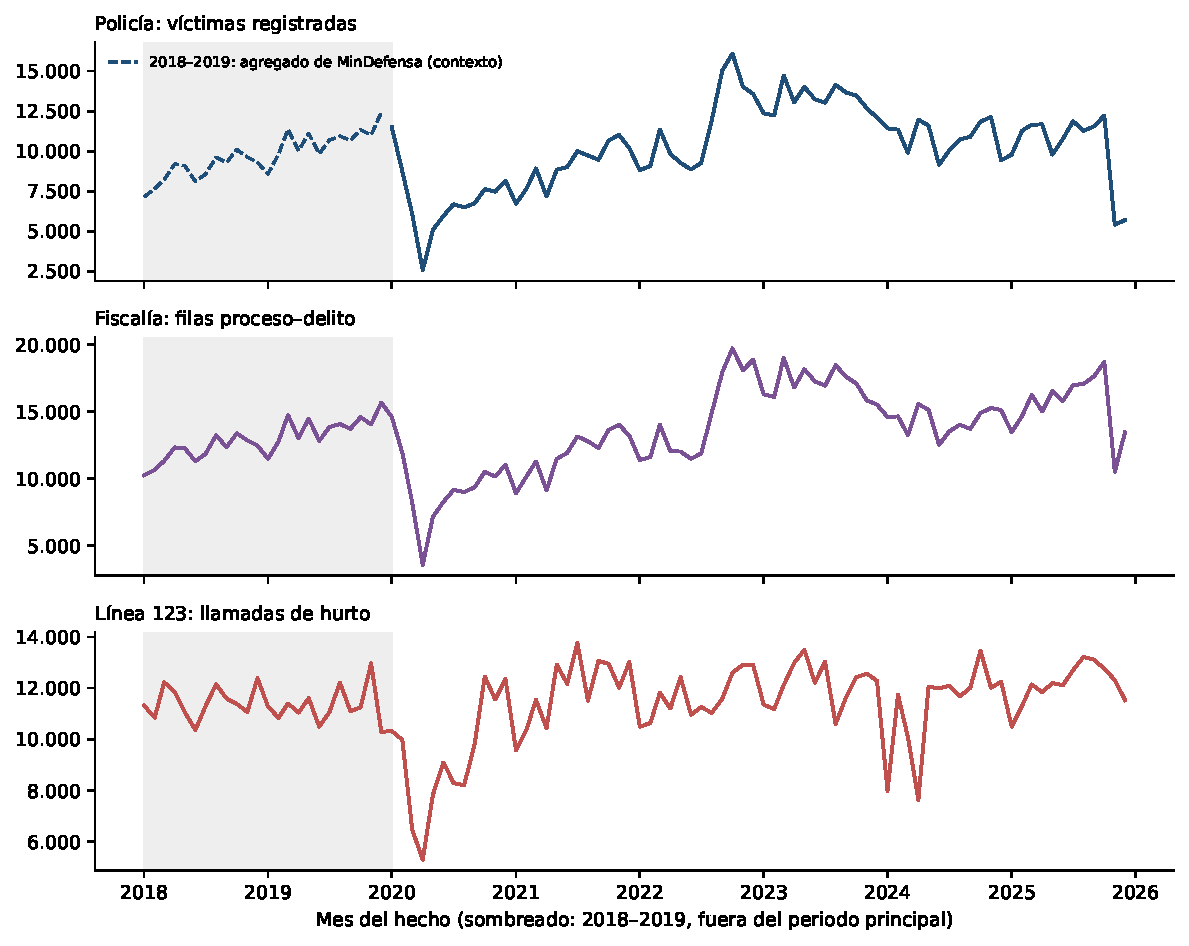
\includegraphics[width=\textwidth]{figuras/series_mensuales_fuentes.pdf}}{\fbox{Figura pendiente: \texttt{figuras/series\_mensuales\_fuentes.pdf}}}
\caption{Series mensuales de las tres fuentes, cada una en su propia unidad. Fuente: \texttt{outputs/informe/series\_mensuales\_fuentes.csv}.}\label{fig:series}
\end{figure}

\subsection{Unidades de observación y posibilidades de integración}

Las tres fuentes describen fenómenos relacionados, pero cada fila representa algo distinto. La tabla~\ref{tab:compatibilidad} resume qué es una fila en cada fuente y con qué resolución temporal y territorial se publica. Las cifras de Línea 123 y Fiscalía provienen de \texttt{outputs/auditoria/}, y las de la Policía, de la auditoría de los seis archivos anuales (\texttt{outputs/auditoria\_policia/}).

{\small
\setlength{\tabcolsep}{4pt}
\begin{longtable}{@{}>{\raggedright\arraybackslash}p{2.6cm}>{\raggedright\arraybackslash}p{4.2cm}>{\raggedright\arraybackslash}p{4.0cm}>{\raggedright\arraybackslash}p{4.2cm}@{}}
\caption{Unidad de observación y granularidad de las fuentes.}\label{tab:compatibilidad}\\
\toprule
\textbf{Característica} & \textbf{Línea 123} & \textbf{Policía Nacional (registro)} & \textbf{Fiscalía (Procesos V3)} \\
\midrule
\endfirsthead
\toprule
\textbf{Característica} & \textbf{Línea 123} & \textbf{Policía Nacional (registro)} & \textbf{Fiscalía (Procesos V3)} \\
\midrule
\endhead
\bottomrule
\endfoot
Qué es una fila & Un agregado de llamadas procedentes por año, mes, localidad, UPZ y tipo de incidente & Un registro con \texttt{CANTIDAD} = 1 que trae el género y el grupo de edad de una persona, es decir, una víctima & Un par proceso--delito (noticia criminal); un mismo proceso puede ocupar varias filas \\
\addlinespace
Medida de conteo & Suma de \texttt{CANT\_INCIDENTES}, no número de filas: 25.144 filas de hurto suman 1.094.313 llamadas (2018--2025) & Número de filas, igual a la suma de \texttt{CANTIDAD}: 741.986 en 2020--2025 & Filas o procesos únicos: 1.300.703 filas y 1.297.042 procesos (2018--2025) \\
\addlinespace
Resolución temporal & Año y mes & Fecha diaria del hecho & Año y mes del hecho (767 filas del total descargado no lo traen); también año y mes de creación del proceso \\
\addlinespace
Resolución territorial & 20 localidades y 116 UPZ, más valores sin ubicación («SIN LOCALIZACION», «SIN UPZ \ldots» y «-»), que suman 121.254 filas de UPZ & Municipio (código DANE); sin localidad ni barrio & Municipio (todo 11001), zona urbana o rural y seccional; sin localidad \\
\addlinespace
Definición de hurto & Tipos de detalle que contienen «hurto»; uno cambia de nombre en 2019 y se homologa por código & \texttt{DELITOS} = «(05022) Hurto a personas» & Capítulo «Del Hurto»: incluye todas las modalidades (personas, automotores, residencias, etc.) \\
\addlinespace
Identificador & \texttt{ID}, no único: 2.633 identificadores repetidos en el archivo completo y 166 en las filas de hurto 2018--2025 & Sin identificador & \texttt{proceso\_anonimizado} \\
\addlinespace
Qué mide & Demanda ciudadana de atención (llamadas) & Hechos denunciados o conocidos por la Policía & Respuesta judicial (procesos abiertos) \\
\end{longtable}
}

\subsubsection{Llaves de integración}

\begin{itemize}
  \item \textbf{Mes $\times$ Bogotá.} Es la única resolución que comparten las tres fuentes: Línea 123 y Fiscalía publican año y mes, y la Policía puede agregarse de día a mes. Sobre esta llave se construirán series paralelas, una por fuente, para comparar tendencias y estudiar desfases (por ejemplo, entre la llamada, el registro policial y la apertura del proceso).
  \item \textbf{Mes $\times$ localidad.} Solo está disponible en Línea 123, así que los análisis territoriales por localidad o UPZ se harán únicamente con esa fuente y no se contrastarán con las otras dos.
  \item \textbf{Día $\times$ Bogotá.} Solo está disponible en la Policía. Permite estudiar estacionalidad semanal y festivos, sin contraparte en las demás fuentes.
\end{itemize}

\subsubsection{Cruces no válidos}

\begin{itemize}
  \item \textbf{Sumar filas o conteos de fuentes distintas.} Una misma situación puede generar una llamada, un registro policial y un proceso, de modo que la suma contaría varias veces el mismo hecho. Tampoco se suman entre fuentes para alcanzar el requisito de 500.000 registros.
  \item \textbf{Enlazar registros individuales.} No hay un identificador común. La Policía no publica identificador y las fuentes no comparten ubicación precisa ni hora, así que no es posible quitar duplicados registro a registro, como en los estudios con microdatos georreferenciados.
  \item \textbf{Comparar territorios sin equivalencia.} Por ejemplo, la distribución por localidad de Línea 123 con el total de la ciudad de las otras fuentes.
  \item \textbf{Equiparar «hurto» entre fuentes sin homologar.} El capítulo «Del Hurto» de la Fiscalía incluye modalidades que no son hurto a personas, y las categorías de Línea 123 son tipificaciones operativas de la llamada.
  \item \textbf{Usar la fecha de creación del proceso como fecha del hecho,} o datos que no estarían disponibles al momento de predecir. Los registros judiciales de un mes pueden completarse meses después, así que su uso como predictor exigirá controlar ese rezago.
\end{itemize}

\subsection{Variable objetivo y conjunto de modelamiento}\label{sec:objetivo}

La variable objetivo es el \textbf{número diario de víctimas de hurto a personas registradas por la Policía Nacional en Bogotá}. Se obtiene contando, para cada fecha del hecho, las filas del registro que pasan los filtros de la tabla~\ref{tab:embudo}. El resultado es una serie de 2.192 días, del 1 de enero de 2020 al 31 de diciembre de 2025, que suma las 741.986 víctimas. Ningún día queda vacío, así que no hay que imputar valores. La tabla~\ref{tab:serie} resume la serie y la figura~\ref{fig:serie} la muestra.

\begin{table}[H]
\centering
\caption{Estadísticas descriptivas de la serie diaria objetivo, 2020--2025.}\label{tab:serie}
\begin{tabular}{@{}lr@{}}
\toprule
\textbf{Estadístico} & \textbf{Valor} \\
\midrule
Días (observaciones del conjunto de modelamiento) & 2.192 \\
Días sin registros & 0 \\
Media de víctimas por día & 338,50 \\
Mediana & 337 \\
Desviación estándar & 115,61 \\
Mínimo & 25 (22 de marzo de 2020) \\
Máximo & 718 (23 de septiembre de 2022) \\
Media del día con más víctimas (viernes) & 398,22 \\
Media del día con menos víctimas (domingo) & 242,29 \\
\bottomrule
\end{tabular}
\end{table}

\begin{figure}[H]
\centering
\IfFileExists{figuras/serie_diaria_policia.pdf}{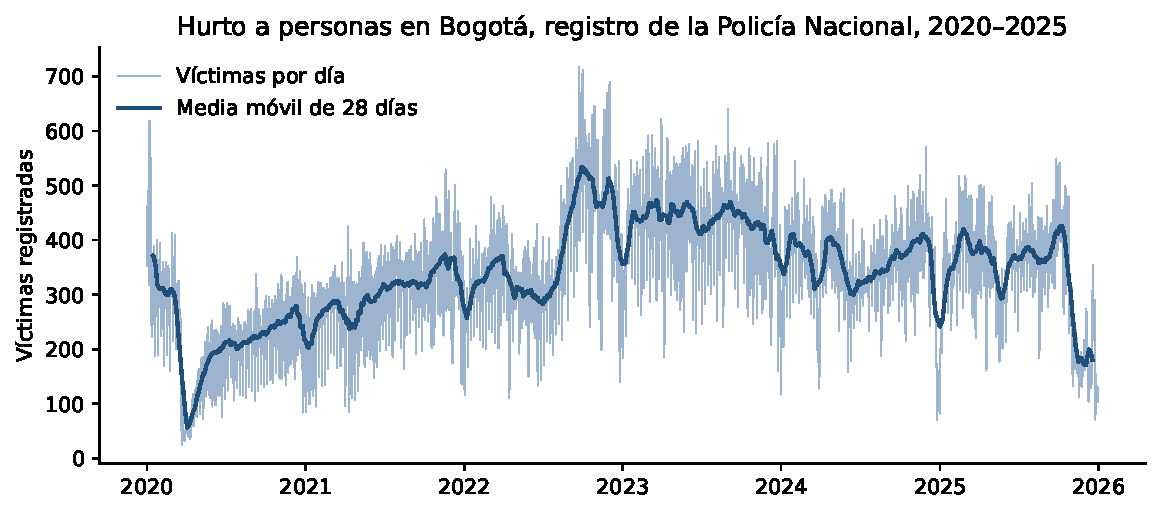
\includegraphics[width=\textwidth]{figuras/serie_diaria_policia.pdf}}{\fbox{Figura pendiente: \texttt{figuras/serie\_diaria\_policia.pdf}}}
\caption{Víctimas diarias de hurto a personas registradas en Bogotá y media móvil de 28 días. Fuente: \texttt{outputs/serie\_objetivo/serie\_diaria\_policia.csv}.}\label{fig:serie}
\end{figure}

La serie muestra cuatro rasgos que el modelamiento deberá tener en cuenta:
\begin{itemize}
  \item un mínimo durante el aislamiento obligatorio de 2020;
  \item una recuperación hasta un máximo en el segundo semestre de 2022;
  \item una estacionalidad semanal marcada, con más registros de martes a sábado que el domingo y el lunes;
  \item la caída de noviembre y diciembre de 2025 descrita en la tabla~\ref{tab:calidad}.
\end{itemize}

Las demás fuentes solo podrán entrar al modelo como variables explicativas si están disponibles antes del día que se pronostica y tienen una justificación metodológica. La Línea 123 y la Fiscalía publican por mes y con rezago, así que su uso en un pronóstico diario exigirá rezagos de al menos un mes. Se evaluará en la segunda entrega.

El pronóstico es para el total de la ciudad. Un pronóstico por localidad no es viable con esta fuente, porque el registro no identifica la localidad.

\subsection{Variables derivadas previstas}

En la segunda entrega se construirán, sobre la serie diaria, variables de calendario (año, mes, día de la semana y festivos), rezagos y estadísticas móviles calculadas solo con observaciones pasadas. Las series de la Línea 123 y de la Fiscalía solo se usarán con el rezago con que estarían disponibles al momento de pronosticar, para evitar filtrar información futura.

Estas variables son propuestas metodológicas, no campos existentes en la base original. Su utilidad real se comprobará mediante el análisis exploratorio y la evaluación de modelos.

\subsection{Criterios previstos de calidad de datos}

Durante el preprocesamiento se comprobarán: \textit{completitud} (nulos y continuidad de fechas), \textit{unicidad} (filas repetidas por fecha y municipio), \textit{validez} (conteos no negativos y formatos), \textit{consistencia territorial} (códigos y nombres), \textit{valores atípicos} (picos o caídas de la serie), y \textit{comparabilidad} (cambios de registro y revisiones de cifras). Los valores extremos no se eliminarán automáticamente, pues pueden corresponder a hechos o circunstancias reales.

También se analizarán localidades ausentes o categorías sin ubicación en las fuentes que las incorporen. Los registros pueden estar afectados por subdenuncia y cambios administrativos \citep{riascos2023}; por ello, las predicciones se interpretarán como proyecciones de conteos registrados y no de la totalidad de eventos ocurridos.

\subsection{Análisis y productos previstos para las siguientes entregas}

La segunda entrega profundizará el análisis exploratorio de la serie objetivo (tendencia, estacionalidad y valores atípicos) y la comparación de tendencias entre fuentes. La tercera comparará modelos de pronóstico de la serie diaria con una línea base estacional ingenua, como repetir el valor del mismo día de la semana anterior, y alternativas como SARIMA, Random Forest y XGBoost.

La evaluación empleará una separación cronológica de entrenamiento y prueba, evitando mezclar observaciones futuras en el entrenamiento. Se considerarán métricas como error absoluto medio (MAE) y raíz del error cuadrático medio (RMSE). Esta sección establece el plan de análisis; \textbf{no presenta preprocesamiento ejecutado, modelos entrenados ni resultados predictivos}, pues estos corresponden a las siguientes entregas.

\subsection{Consideraciones éticas y limitaciones}

El proyecto utilizará fuentes públicas anonimizadas y no elaborará perfiles individuales. La identificación de zonas con mayores conteos no implica que sus habitantes sean responsables de los delitos. Las diferencias territoriales pueden reflejar, entre otros factores, densidad de población, actividades económicas, población flotante, subregistro o calidad de localización. Por tanto, se evitarán conclusiones causales o estigmatizantes y se documentarán los límites de extrapolación de los modelos.
